% Figura do Cap. II: janela deslizante de estimação e reavaliação das ordens.
% Criada em 05/11/2026, a pedido do autor, junto com a linha do tempo dos
% períodos. Esquema ilustrativo: a janela real tem 120 ou 240 pregões (input
% Janela_Estimacao) e as ordens são reavaliadas a cada 21 pregões (input de
% reseleção do robos/ARIMA-GARCH/ARIMA_GARCH_EA.mq5), como diz o Cap. II.
% PROPOSTA, fora do TG até o autor decidir. Compilada pelo Makefile desta pasta.
\documentclass[10pt,border=2pt]{standalone}
\usepackage[T1]{fontenc}
\usepackage[utf8]{inputenc}
\usepackage{mathptmx}
\usepackage{tikz}
\usetikzlibrary{arrows.meta,patterns,decorations.pathreplacing,calc}
\tikzset{
  dia/.style={draw, minimum size=5mm, inner sep=0pt},
  jan/.style={dia, fill=gray!35},
  hoje/.style={dia, very thick, pattern=north east lines, pattern color=gray!70},
  futuro/.style={dia, dashed, draw=gray},
  fora/.style={dia, draw=gray, text=gray},
  seta/.style={-{Stealth[length=2mm]}, semithick},
  txt/.style={font=\footnotesize, align=center},
}
% \linha{y}{primeiro dia da janela}{rótulo da linha}
\newcommand{\linha}[3]{%
  \node[anchor=east, font=\small, align=right] at (-0.2, #1) {#3};
  \foreach \i in {1,...,16} {
    \pgfmathtruncatemacro{\ini}{#2}
    \pgfmathtruncatemacro{\fim}{#2+10}
    \ifnum\i<\ini \node[fora] (d#2-\i) at (\i*0.5, #1) {};
    \else\ifnum\i>\fim
      \ifnum\i=\numexpr\fim+1\relax \node[hoje] (d#2-\i) at (\i*0.5, #1) {};
      \else \node[futuro] (d#2-\i) at (\i*0.5, #1) {}; \fi
    \else \node[jan] (d#2-\i) at (\i*0.5, #1) {}; \fi\fi}}
\begin{document}
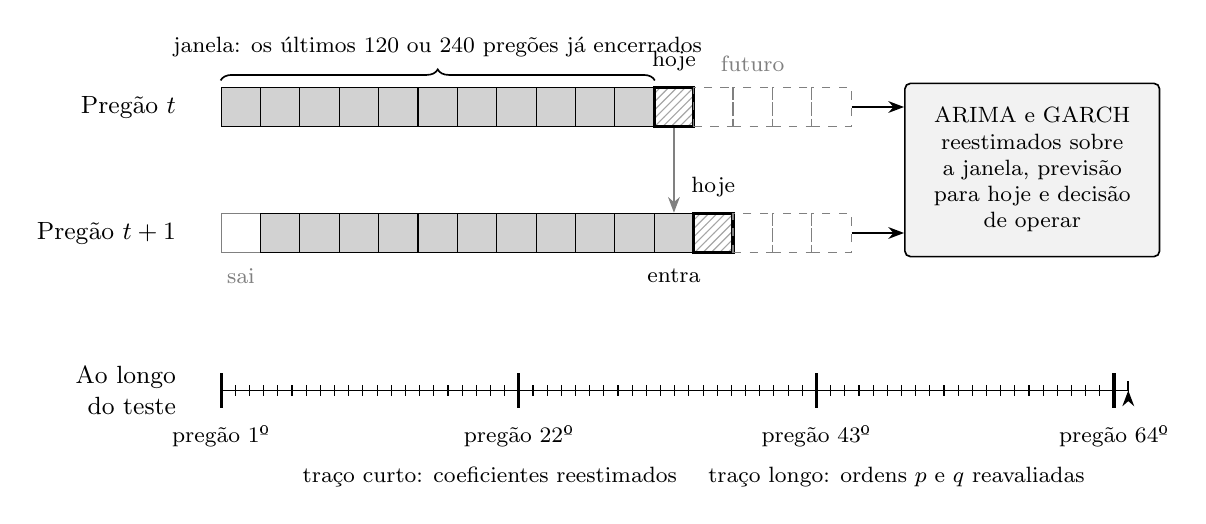
\begin{tikzpicture}
  \linha{0}{1}{Pregão $t$}
  \linha{-1.6}{2}{Pregão $t+1$}

  \draw[decorate, decoration={brace, amplitude=4pt}, semithick]
    ($(d1-1.north west)+(0,0.08)$) -- ($(d1-11.north east)+(0,0.08)$)
    node[midway, above=5pt, txt] {janela: os últimos 120 ou 240 pregões já encerrados};
  \node[txt, above=2pt] at (d1-12.north) {hoje};
  \node[txt, above=2pt, text=gray] at (d1-14.north) {futuro};

  \node[txt, below=2pt, text=gray] at (d2-1.south) {sai};
  \node[txt, below=2pt] at (d2-12.south) {entra};
  \node[txt, above=2pt] at (d2-13.north) {hoje};
  \draw[seta, gray] (d1-12.south) -- (d2-12.north);

  % o que acontece em cada pregão
  \node[draw, semithick, rounded corners=2pt, fill=gray!10, txt, text width=30mm, minimum height=22mm]
    (est) at (10.55, -0.8)
    {ARIMA e GARCH\\reestimados sobre\\a janela, previsão\\para hoje e decisão\\de operar};
  \draw[seta] (d1-16.east) -- (d1-16.east -| est.west);
  \draw[seta] (d2-16.east) -- (d2-16.east -| est.west);

  % ao longo do teste: coeficientes todo dia, ordens a cada 21 pregões
  \begin{scope}[shift={(0.25,-3.6)}]
    \node[anchor=east, font=\small, align=right] at (-0.45, 0) {Ao longo\\do teste};
    \draw[semithick] (0, 0) -- (11.52, 0);
    \foreach \i in {0,...,64} \draw (\i*0.18, -0.07) -- (\i*0.18, 0.07);
    \foreach \i/\r in {0/{1º}, 21/{22º}, 42/{43º}, 63/{64º}} {
      \draw[very thick] (\i*0.18, -0.22) -- (\i*0.18, 0.22);
      \node[txt, below=3pt] at (\i*0.18, -0.22) {pregão \r};}
    \draw[seta] (11.52, 0) -- (11.52, 0);
    \node[txt, anchor=north] at (6.0, -0.85) {traço curto: coeficientes reestimados \quad traço longo: ordens $p$ e $q$ reavaliadas};
  \end{scope}
\end{tikzpicture}
\end{document}
